%%%%%%%%%%%%%%%%%%%%%%%%%%%%%%%%%%%%%%%%%%%%%%%%%%%%%%%%%%%%%%%%%%%%%%%%%%%
\begin{figure*}[tbph!]
\centering
\begin{tabular}{ccc}
\begin{tabular}{ccc}
\subfloat[Fig:][Human Caused Disaster]{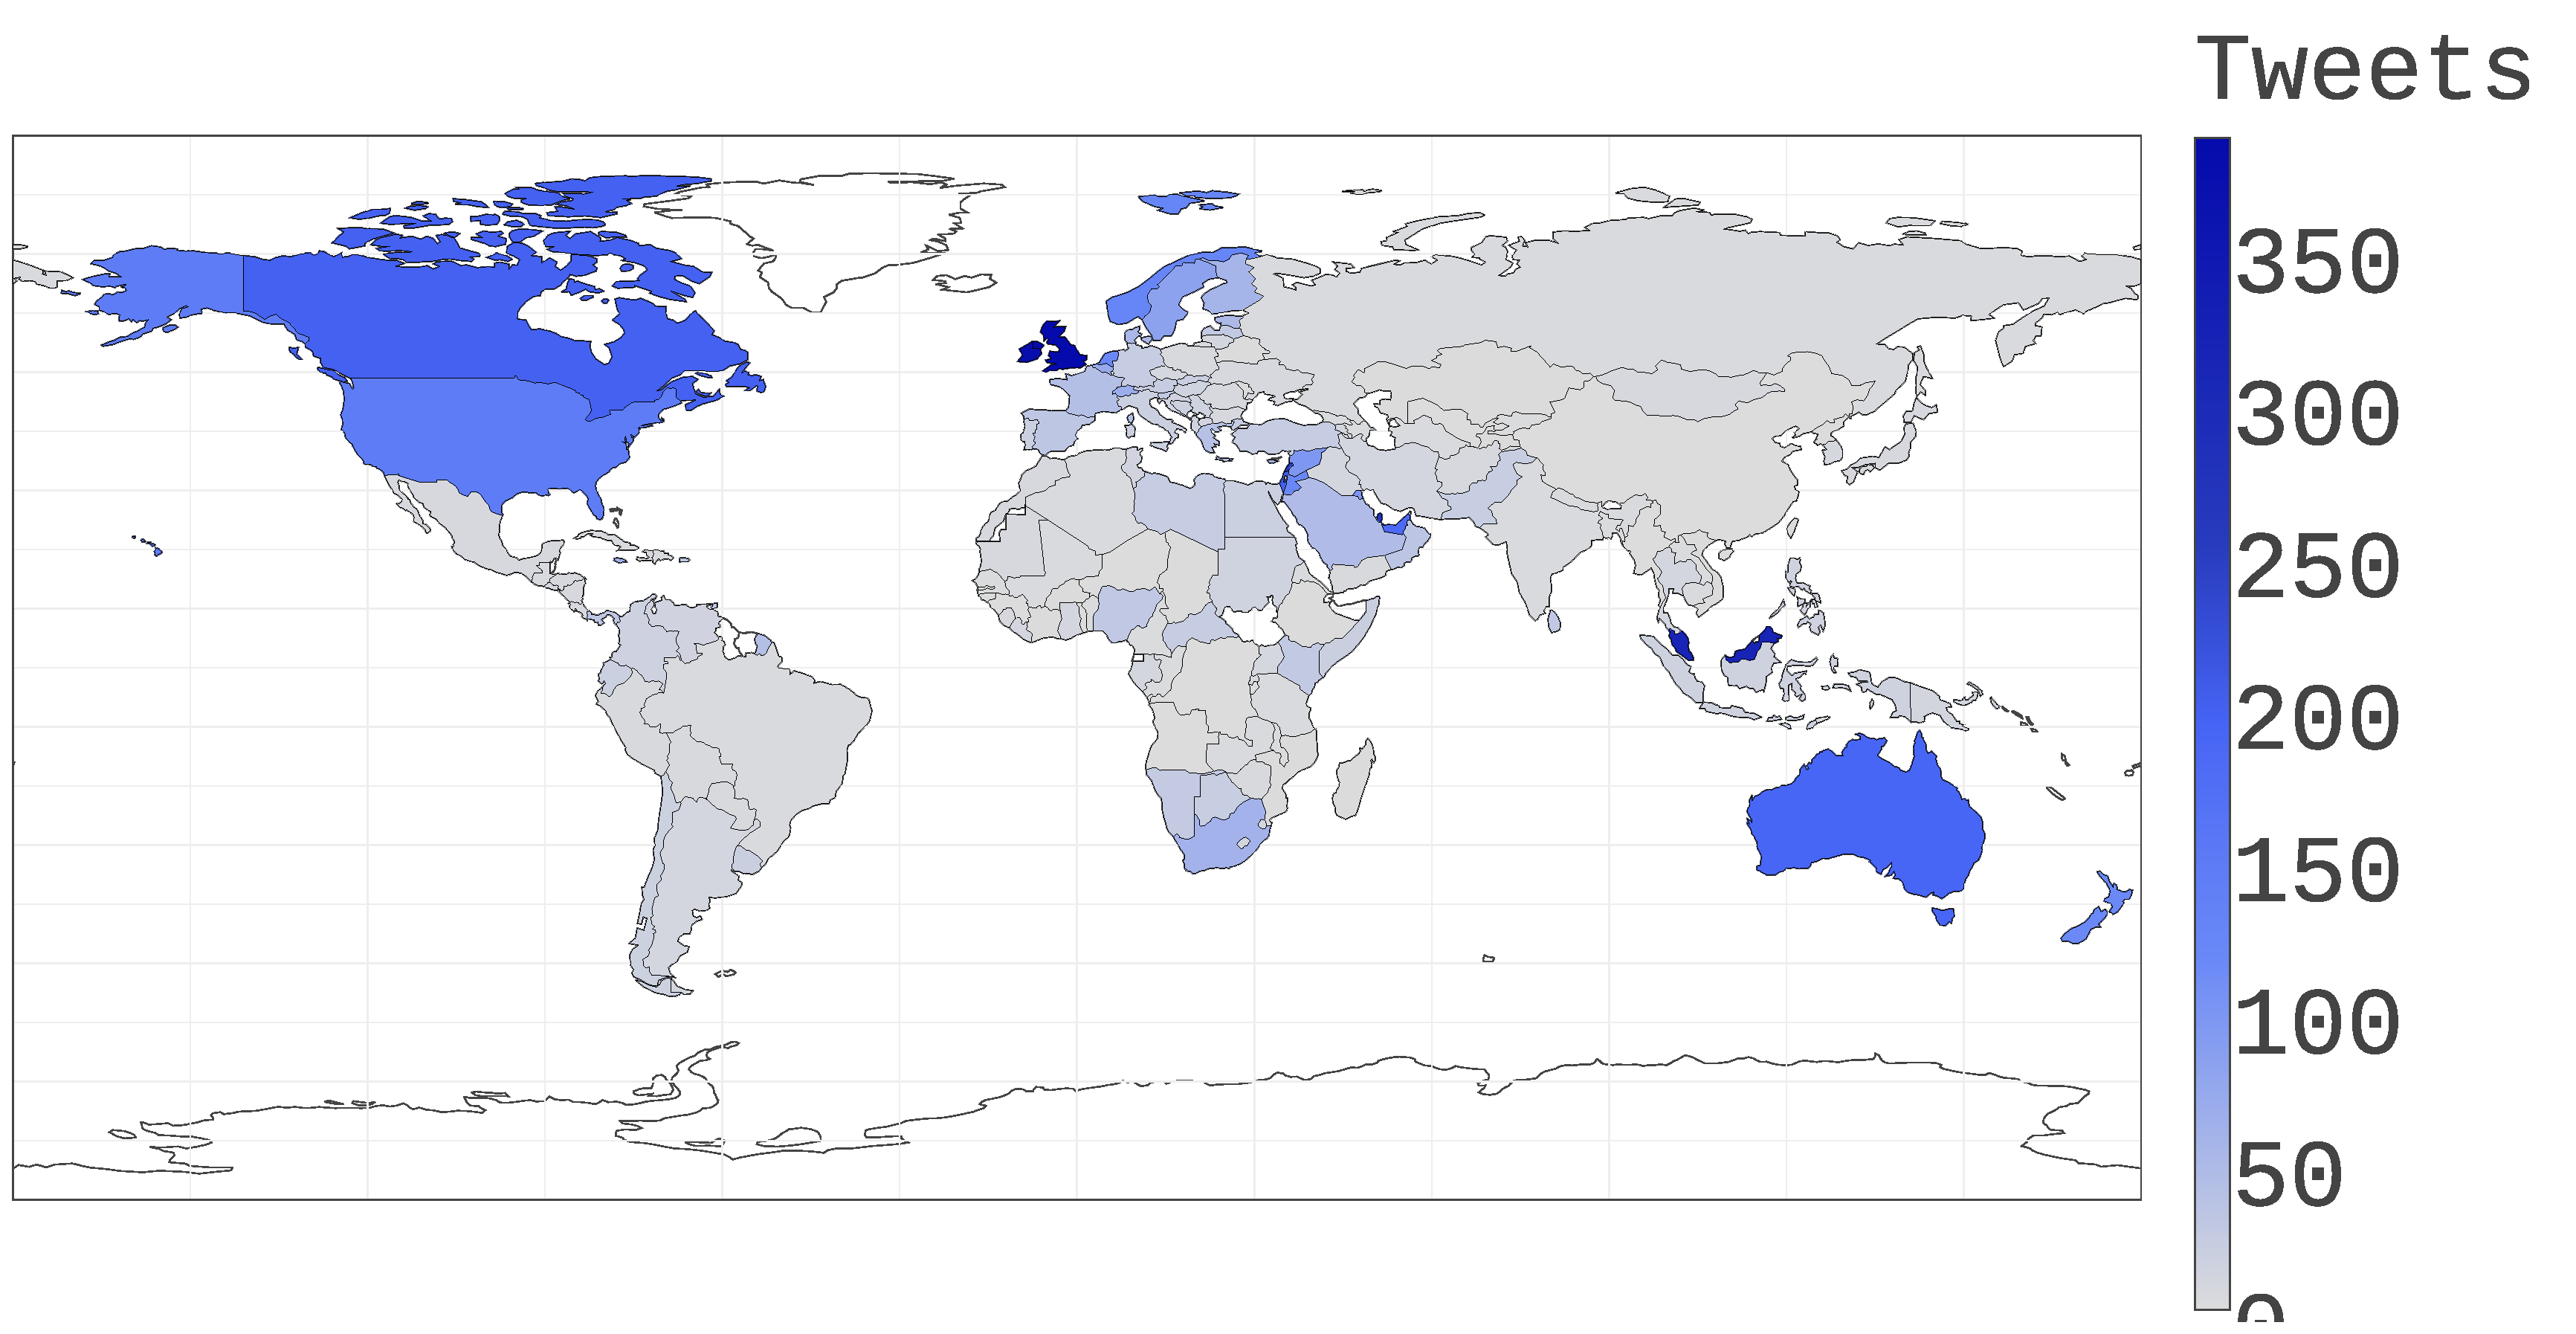
\includegraphics[width=5.3cm]{images/location/world/socialsensor-world-HumanCausedDisaster_location.eps}}
\subfloat[Fig:][Iran Deal]{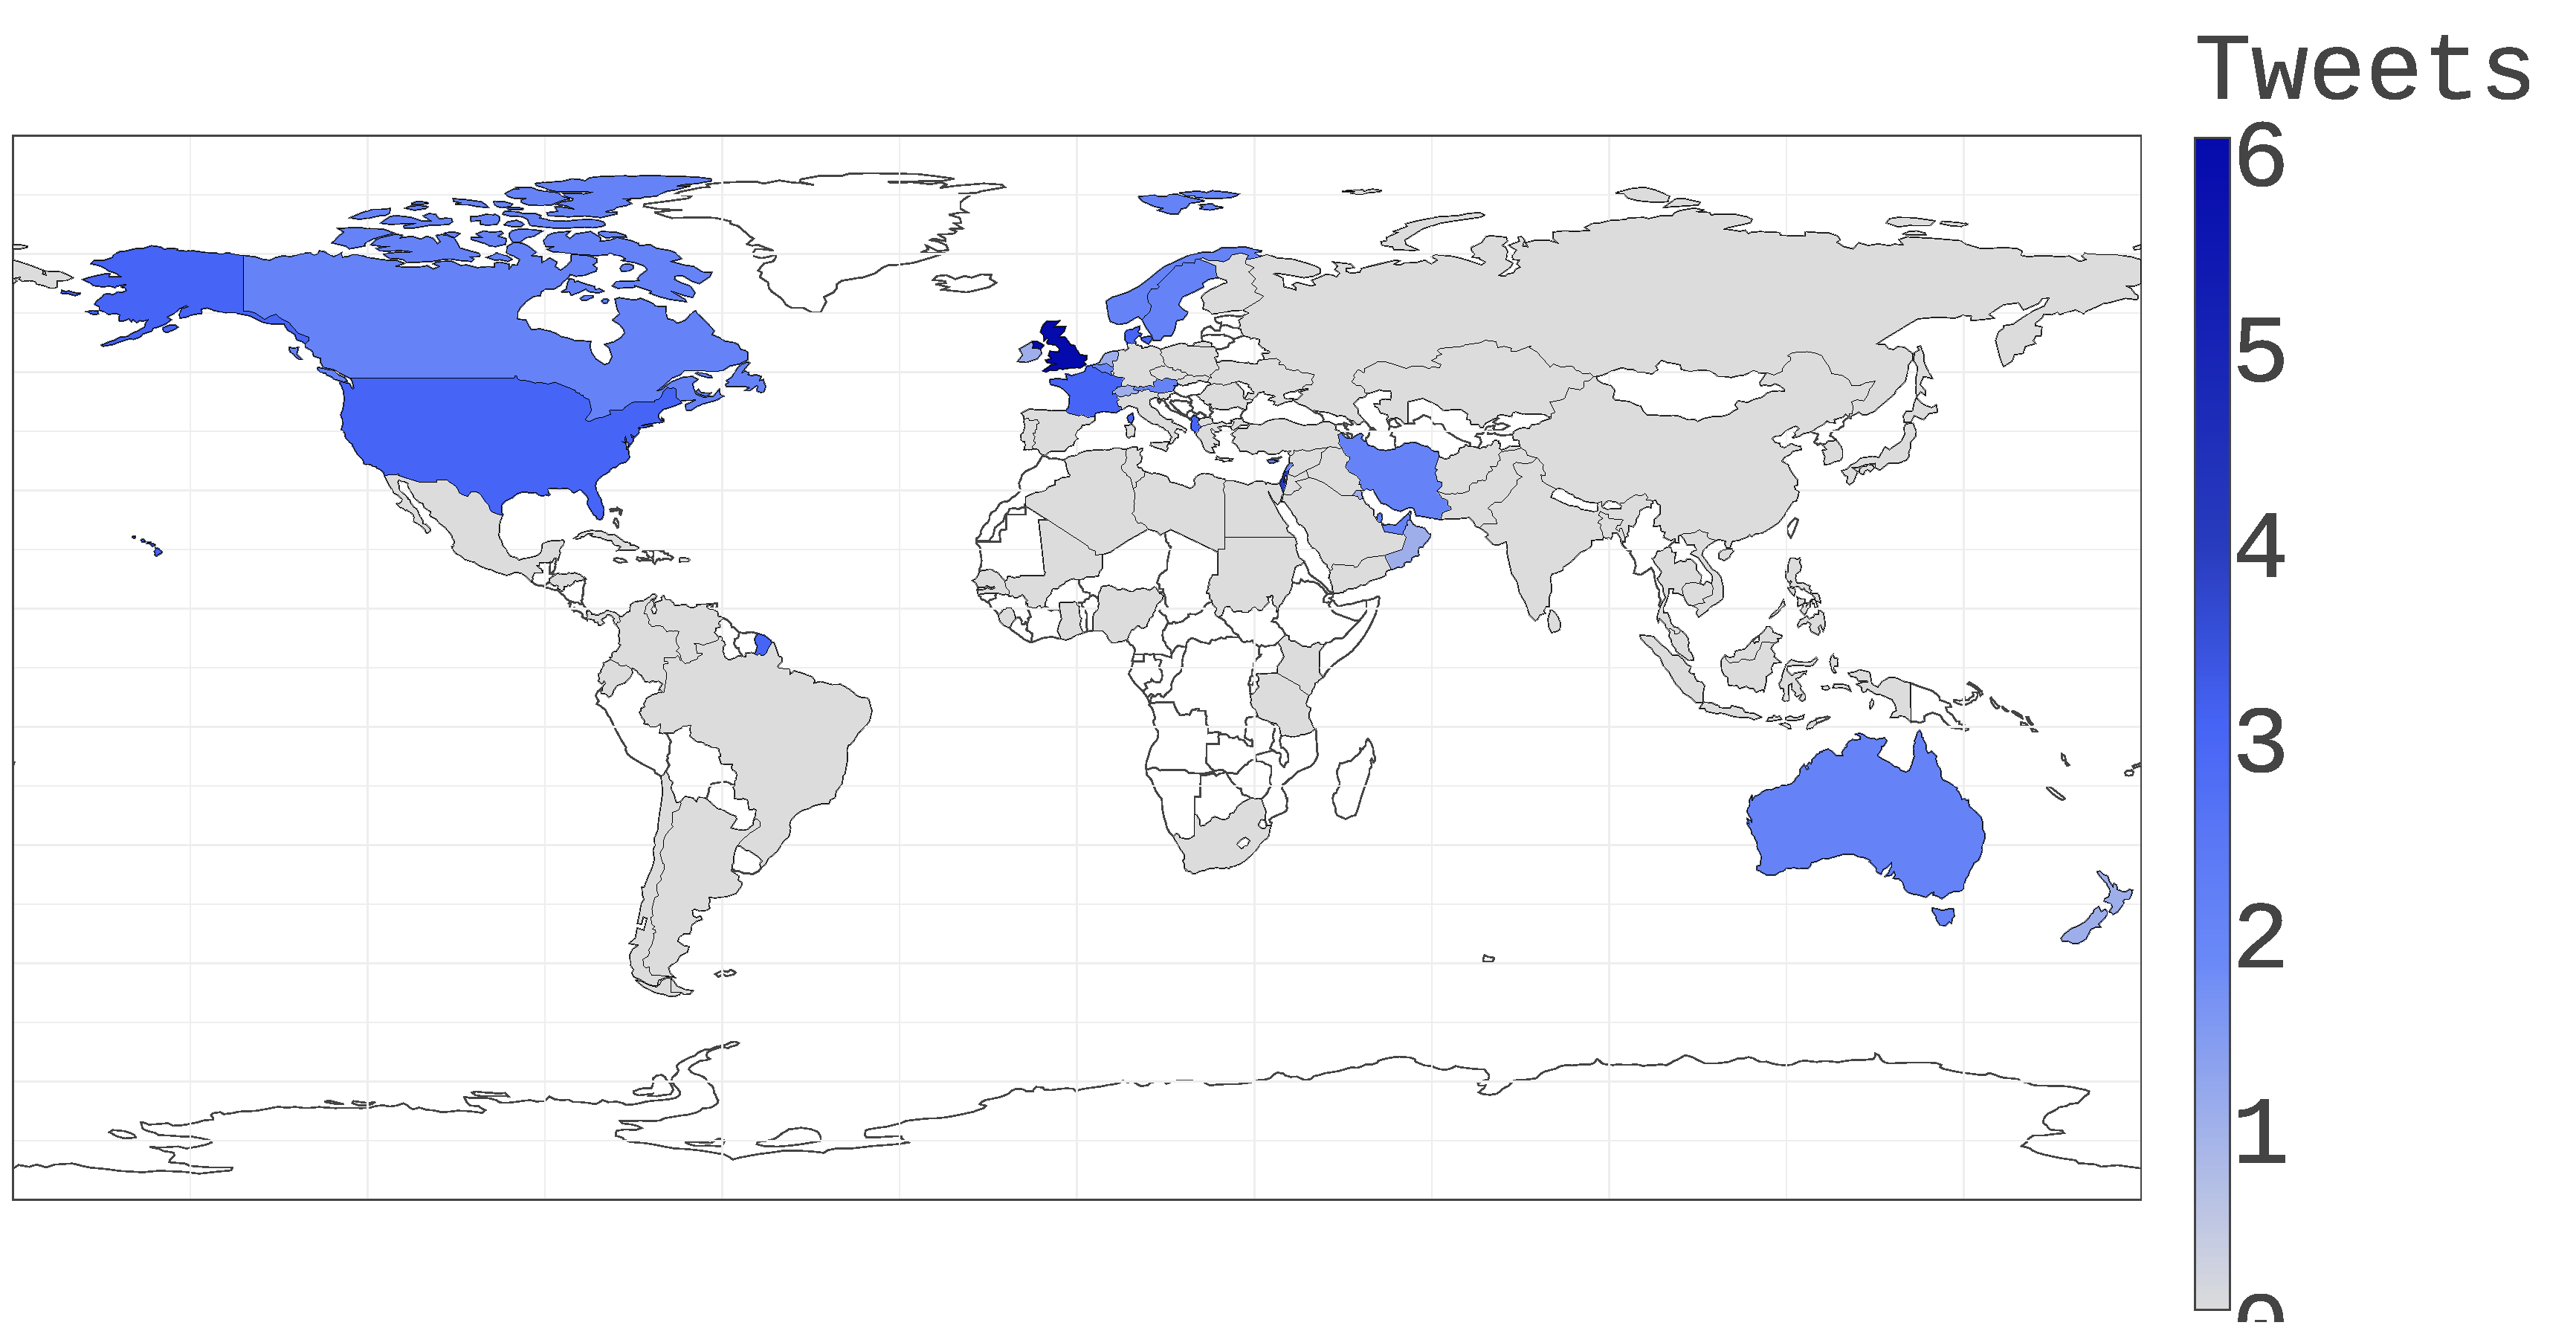
\includegraphics[width=5.3cm]{images/location/world/socialsensor-world-irannucleardeal_location.eps}}
\subfloat[Fig:][Soccer]{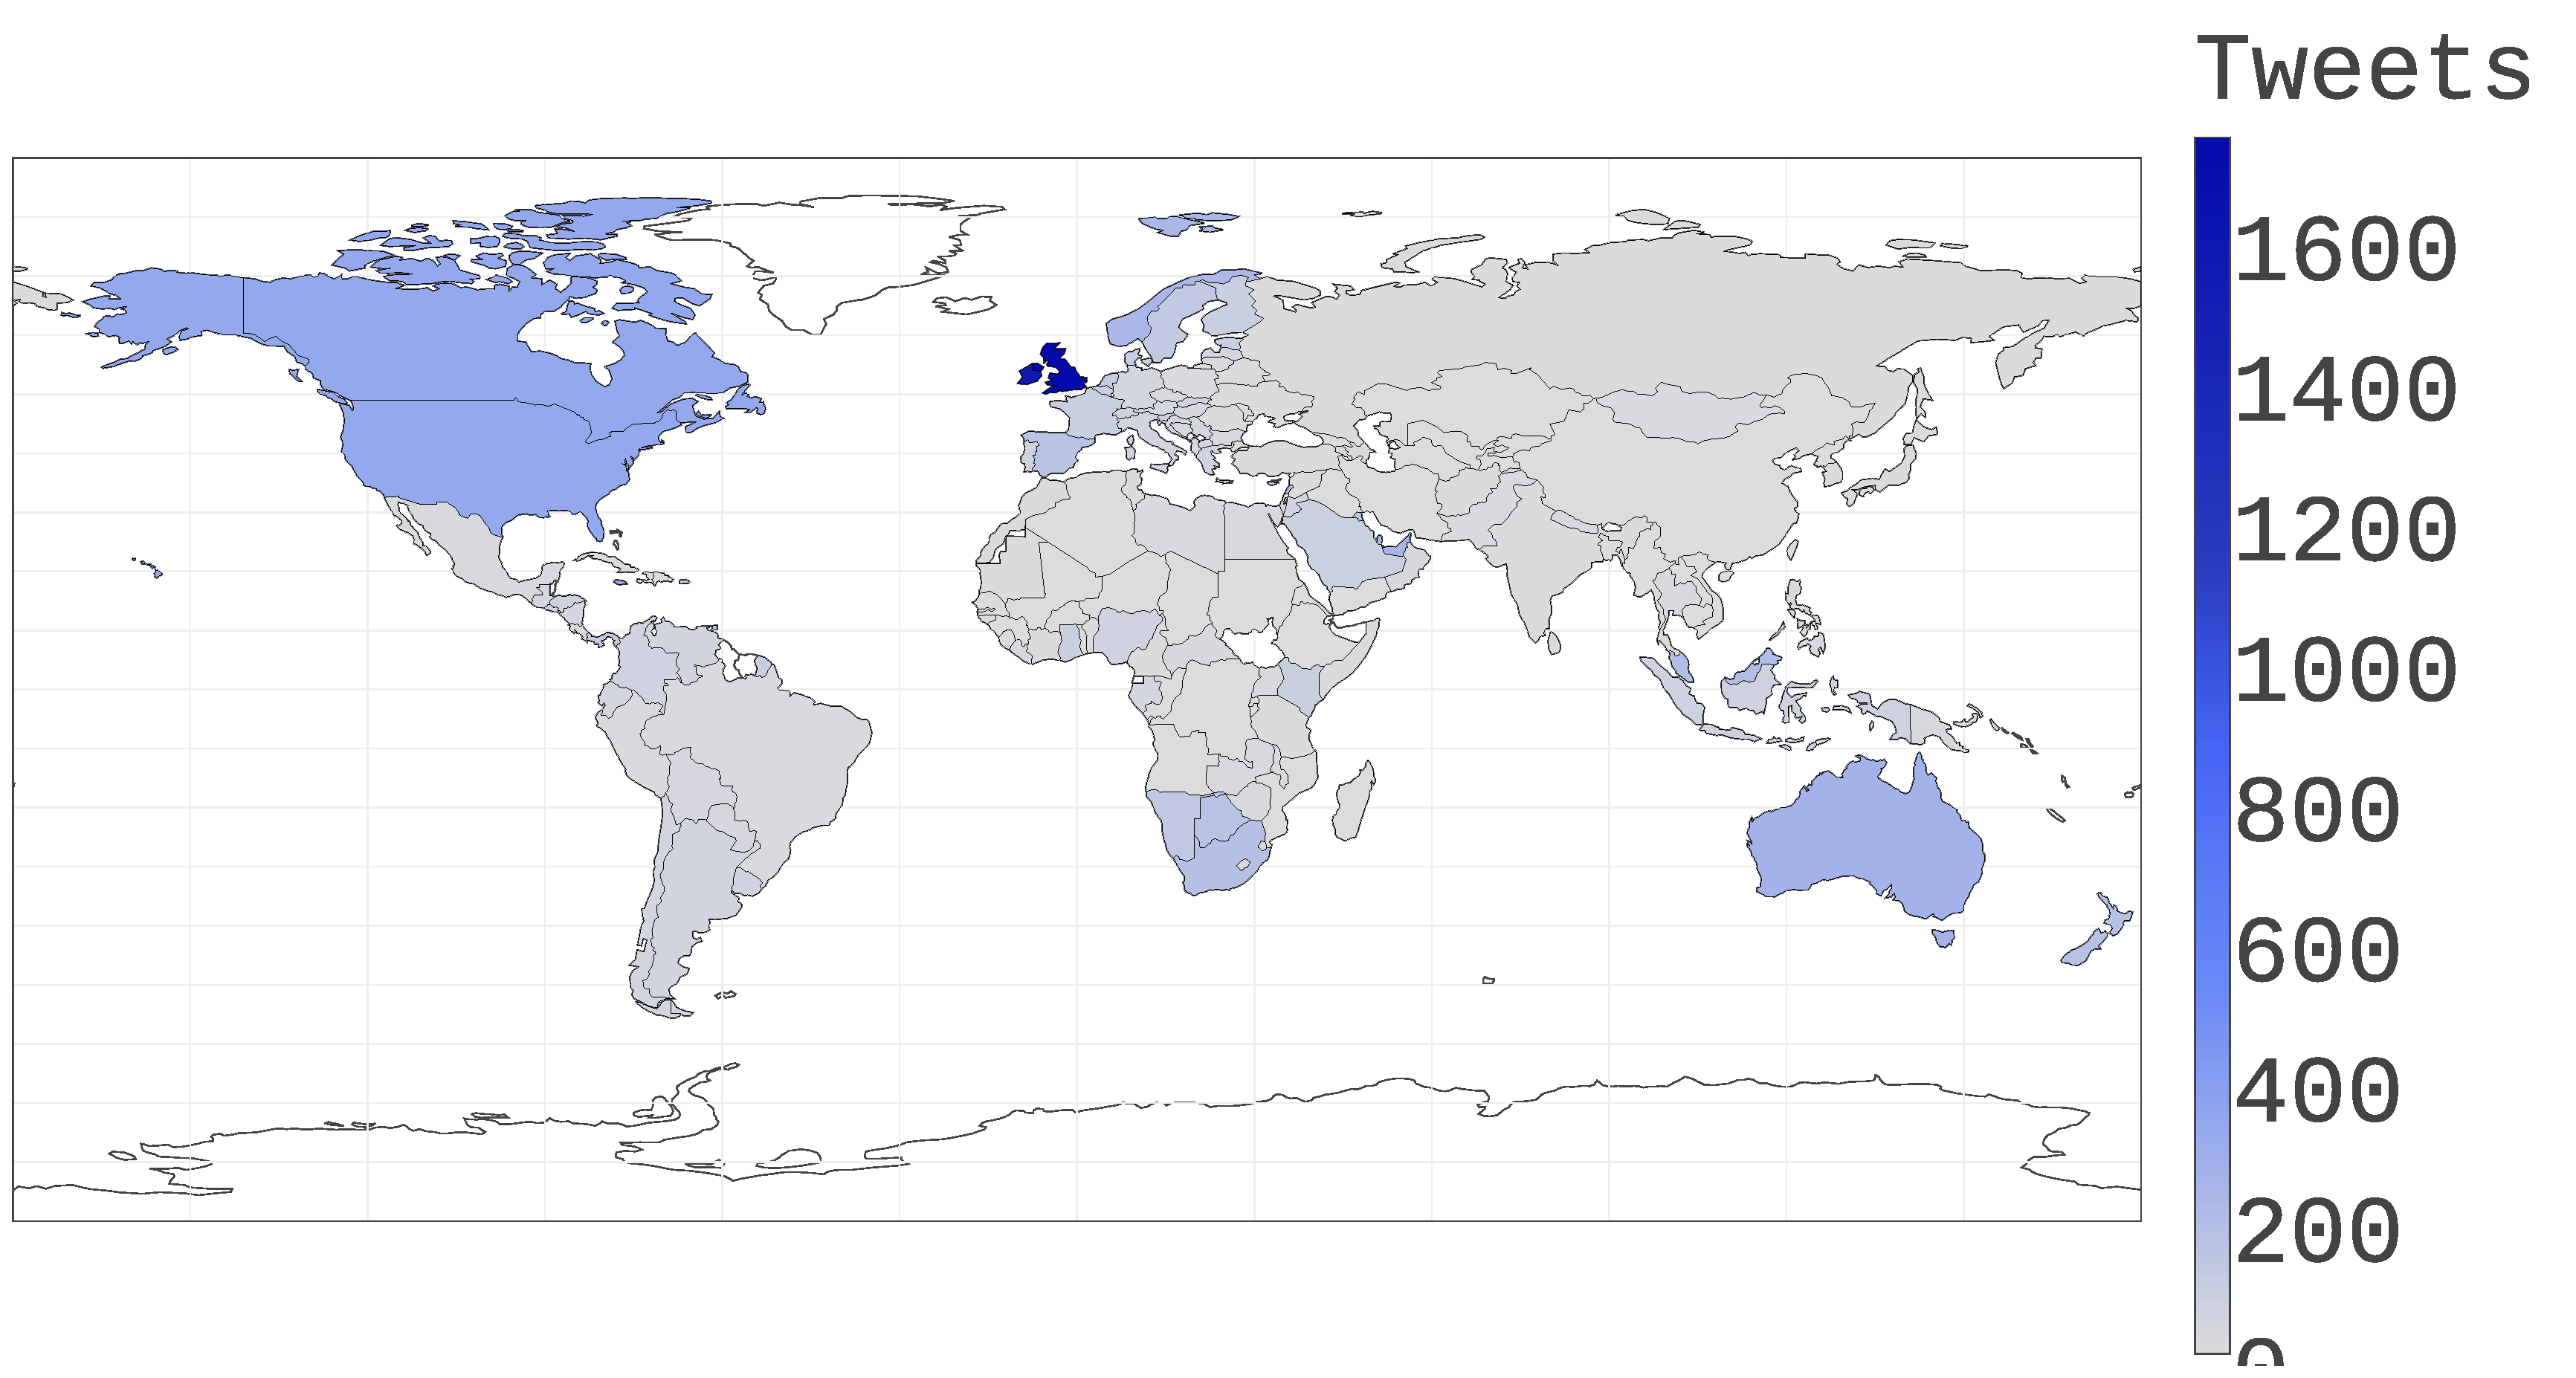
\includegraphics[width=5.3cm]{images/location/world/socialsensor-world-soccer_location.eps}} \\
%\vspace{-10mm}
\subfloat[Fig:][Health Epidemics]{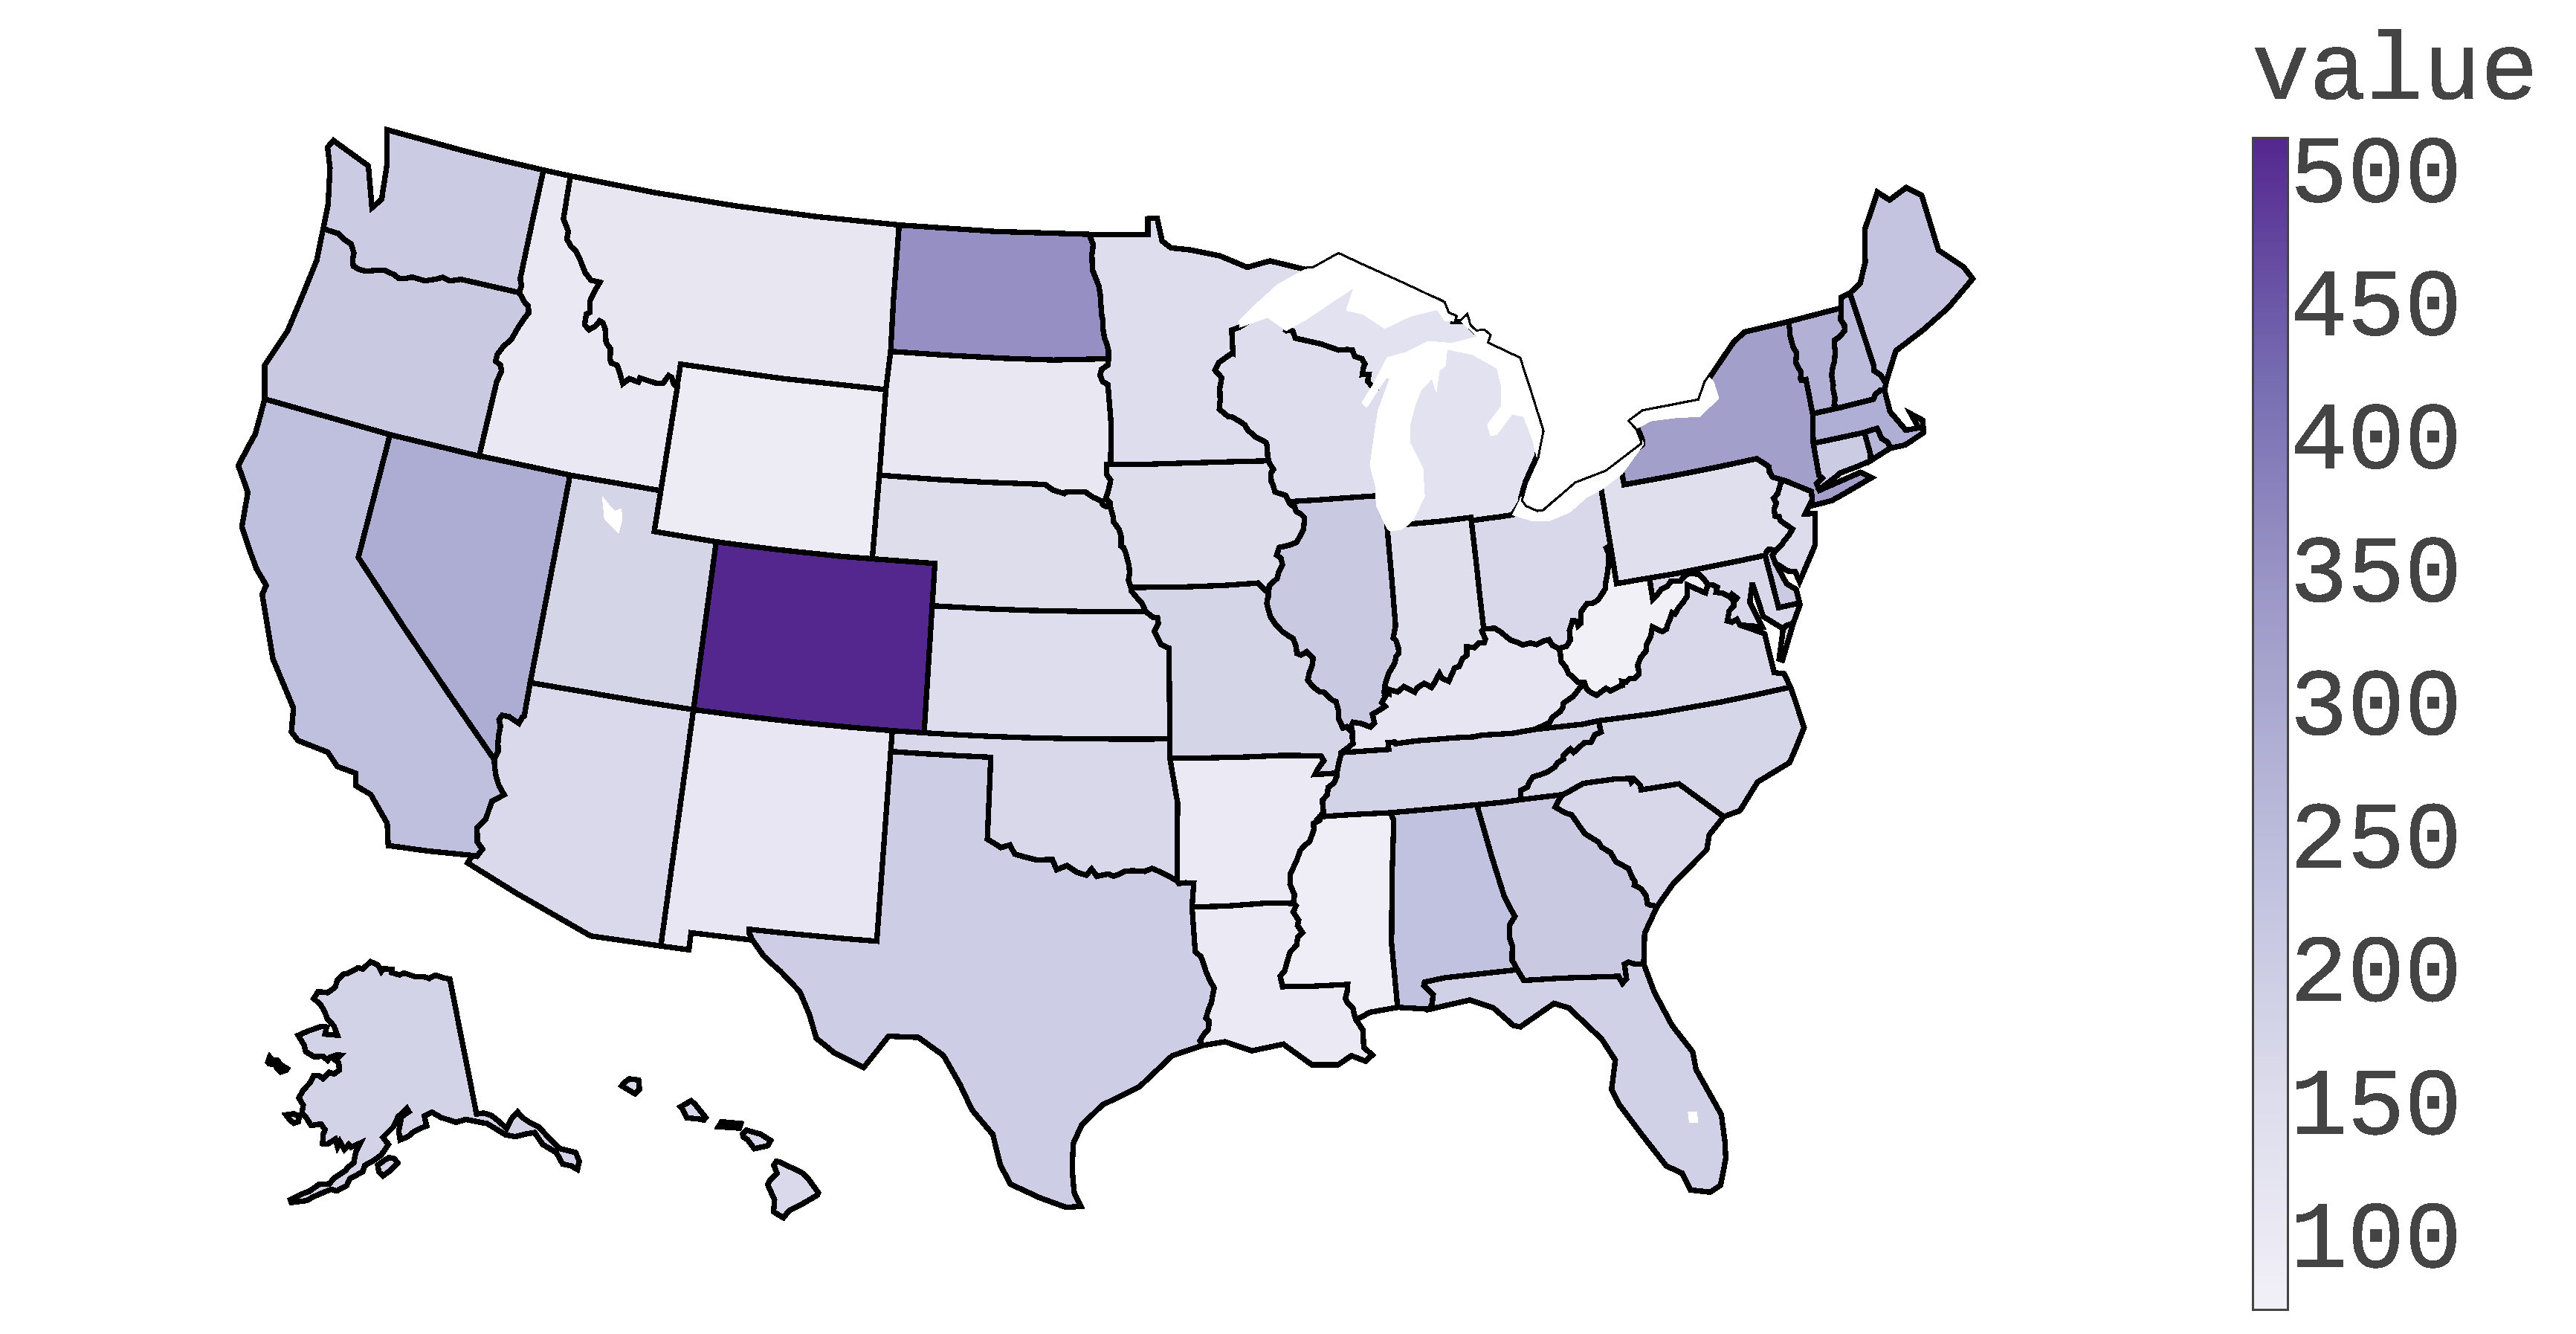
\includegraphics[width=5.3cm]{images/location/states/SocialSensor-us-states-health_epidemics_location.eps}}
\subfloat[Fig:][Social Issues]{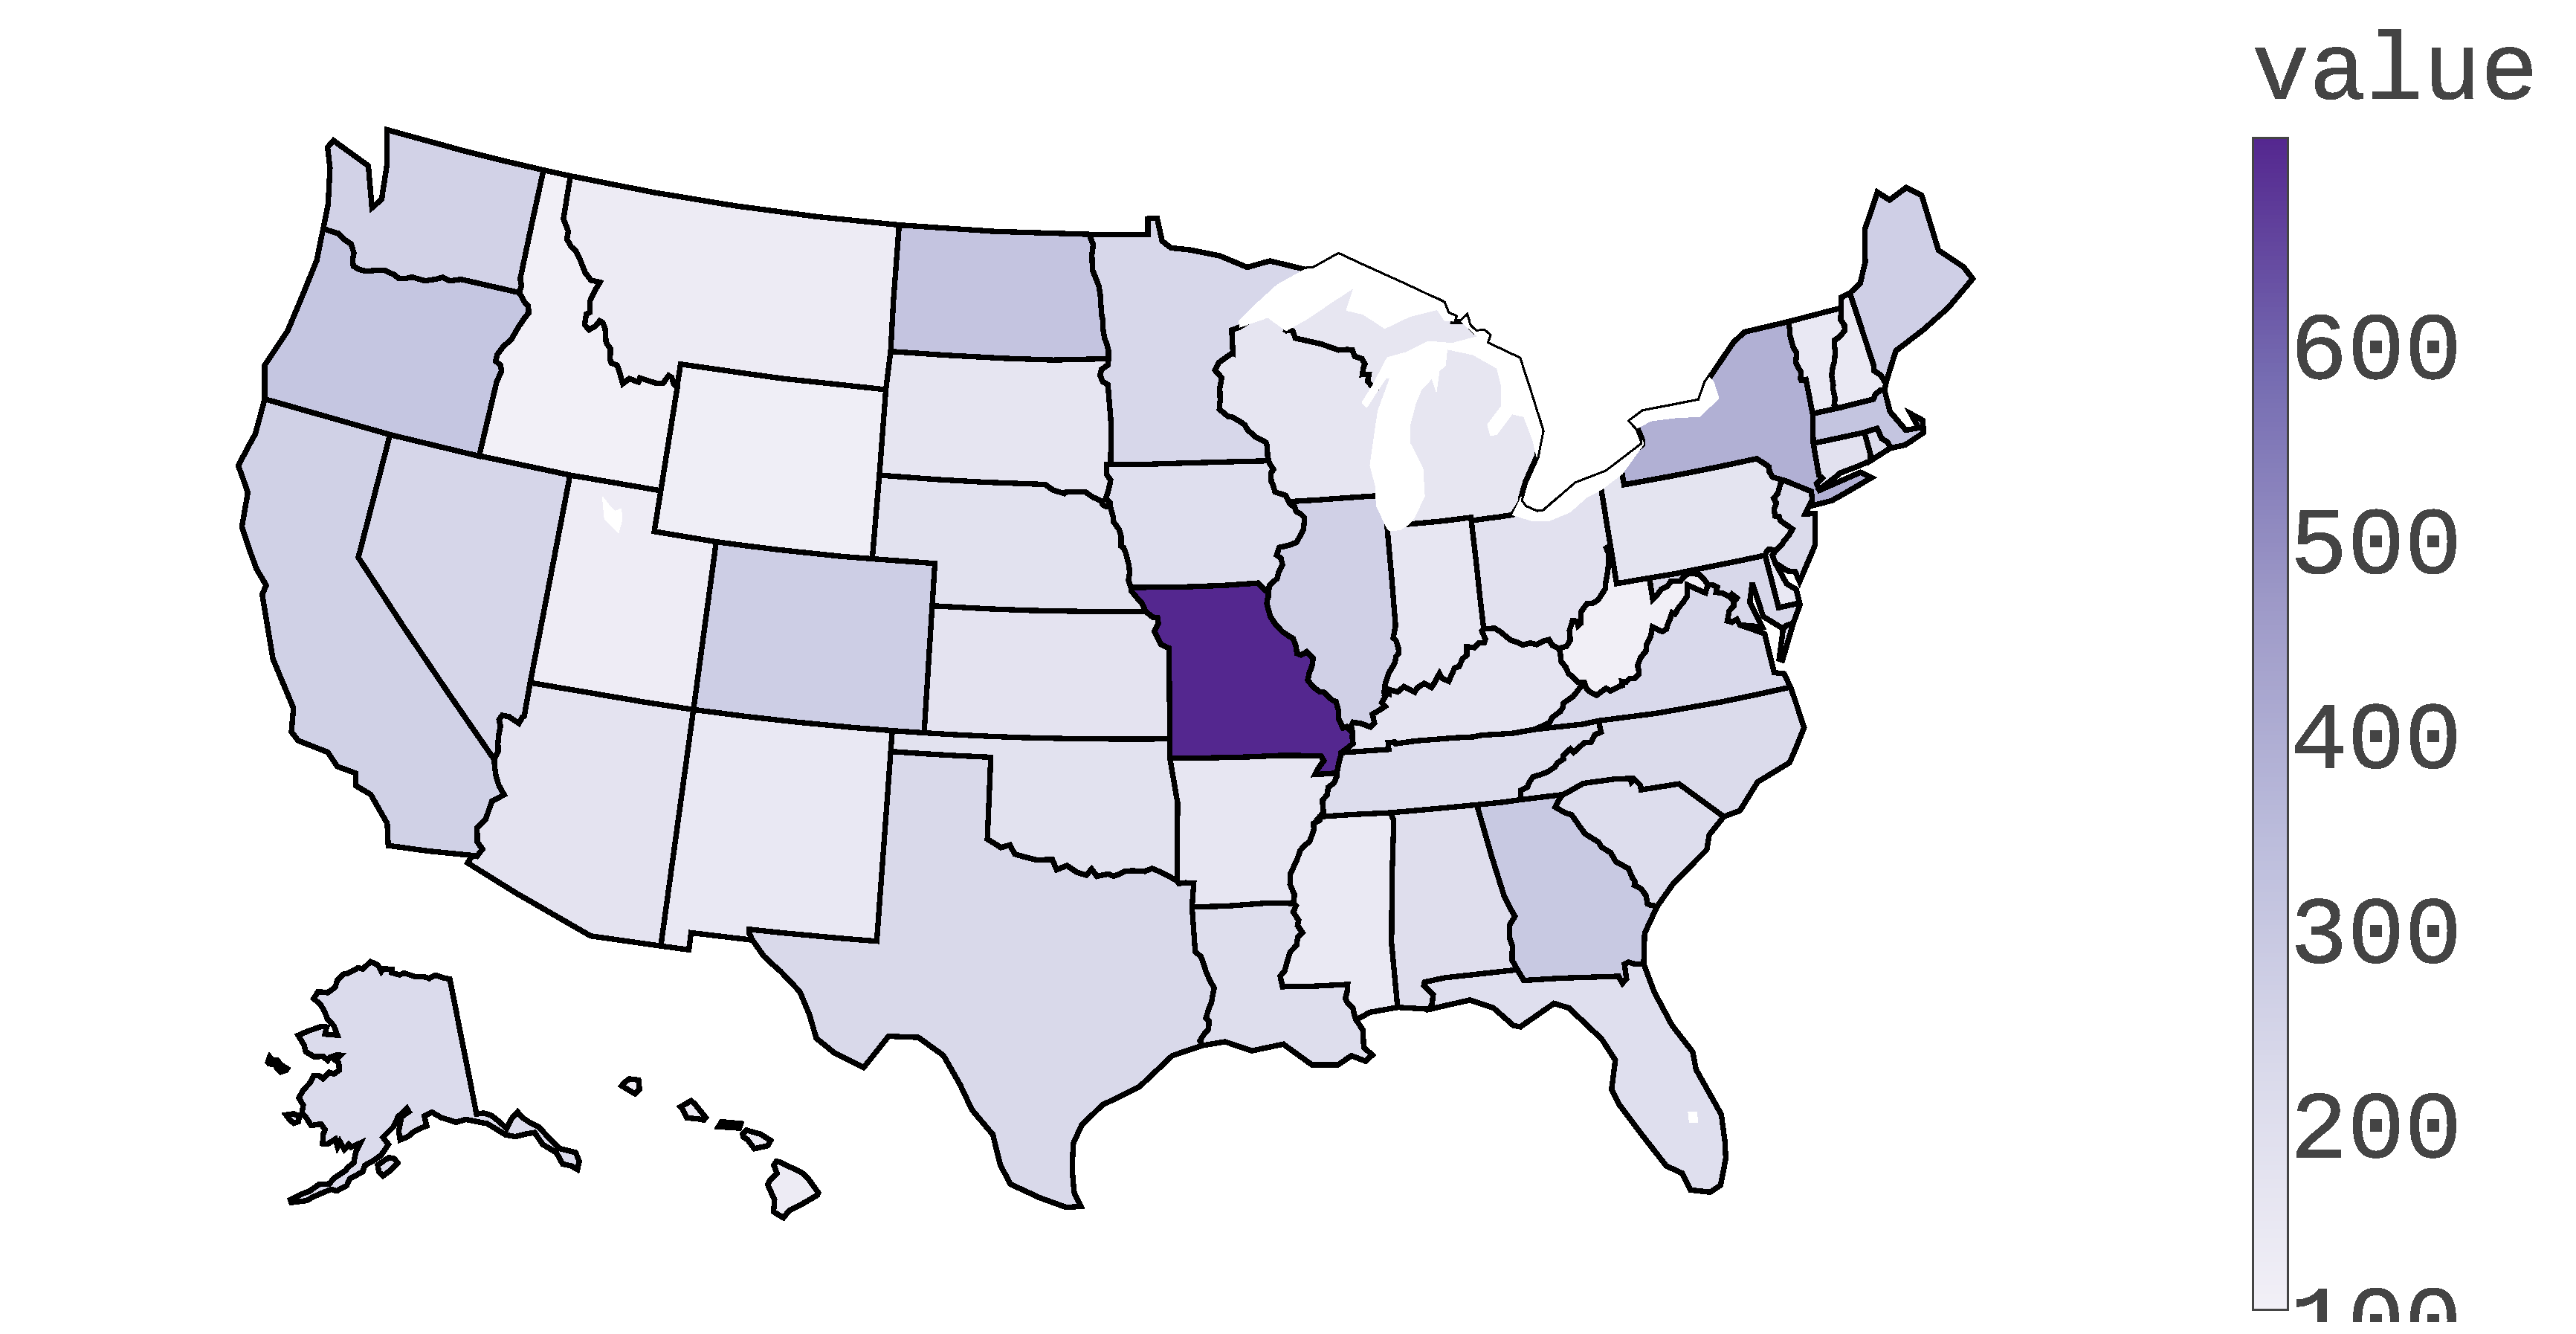
\includegraphics[width=5.3cm]{images/location/states/SocialSensor-us-states-socialissues_location.eps}}
\subfloat[Fig:][Space]{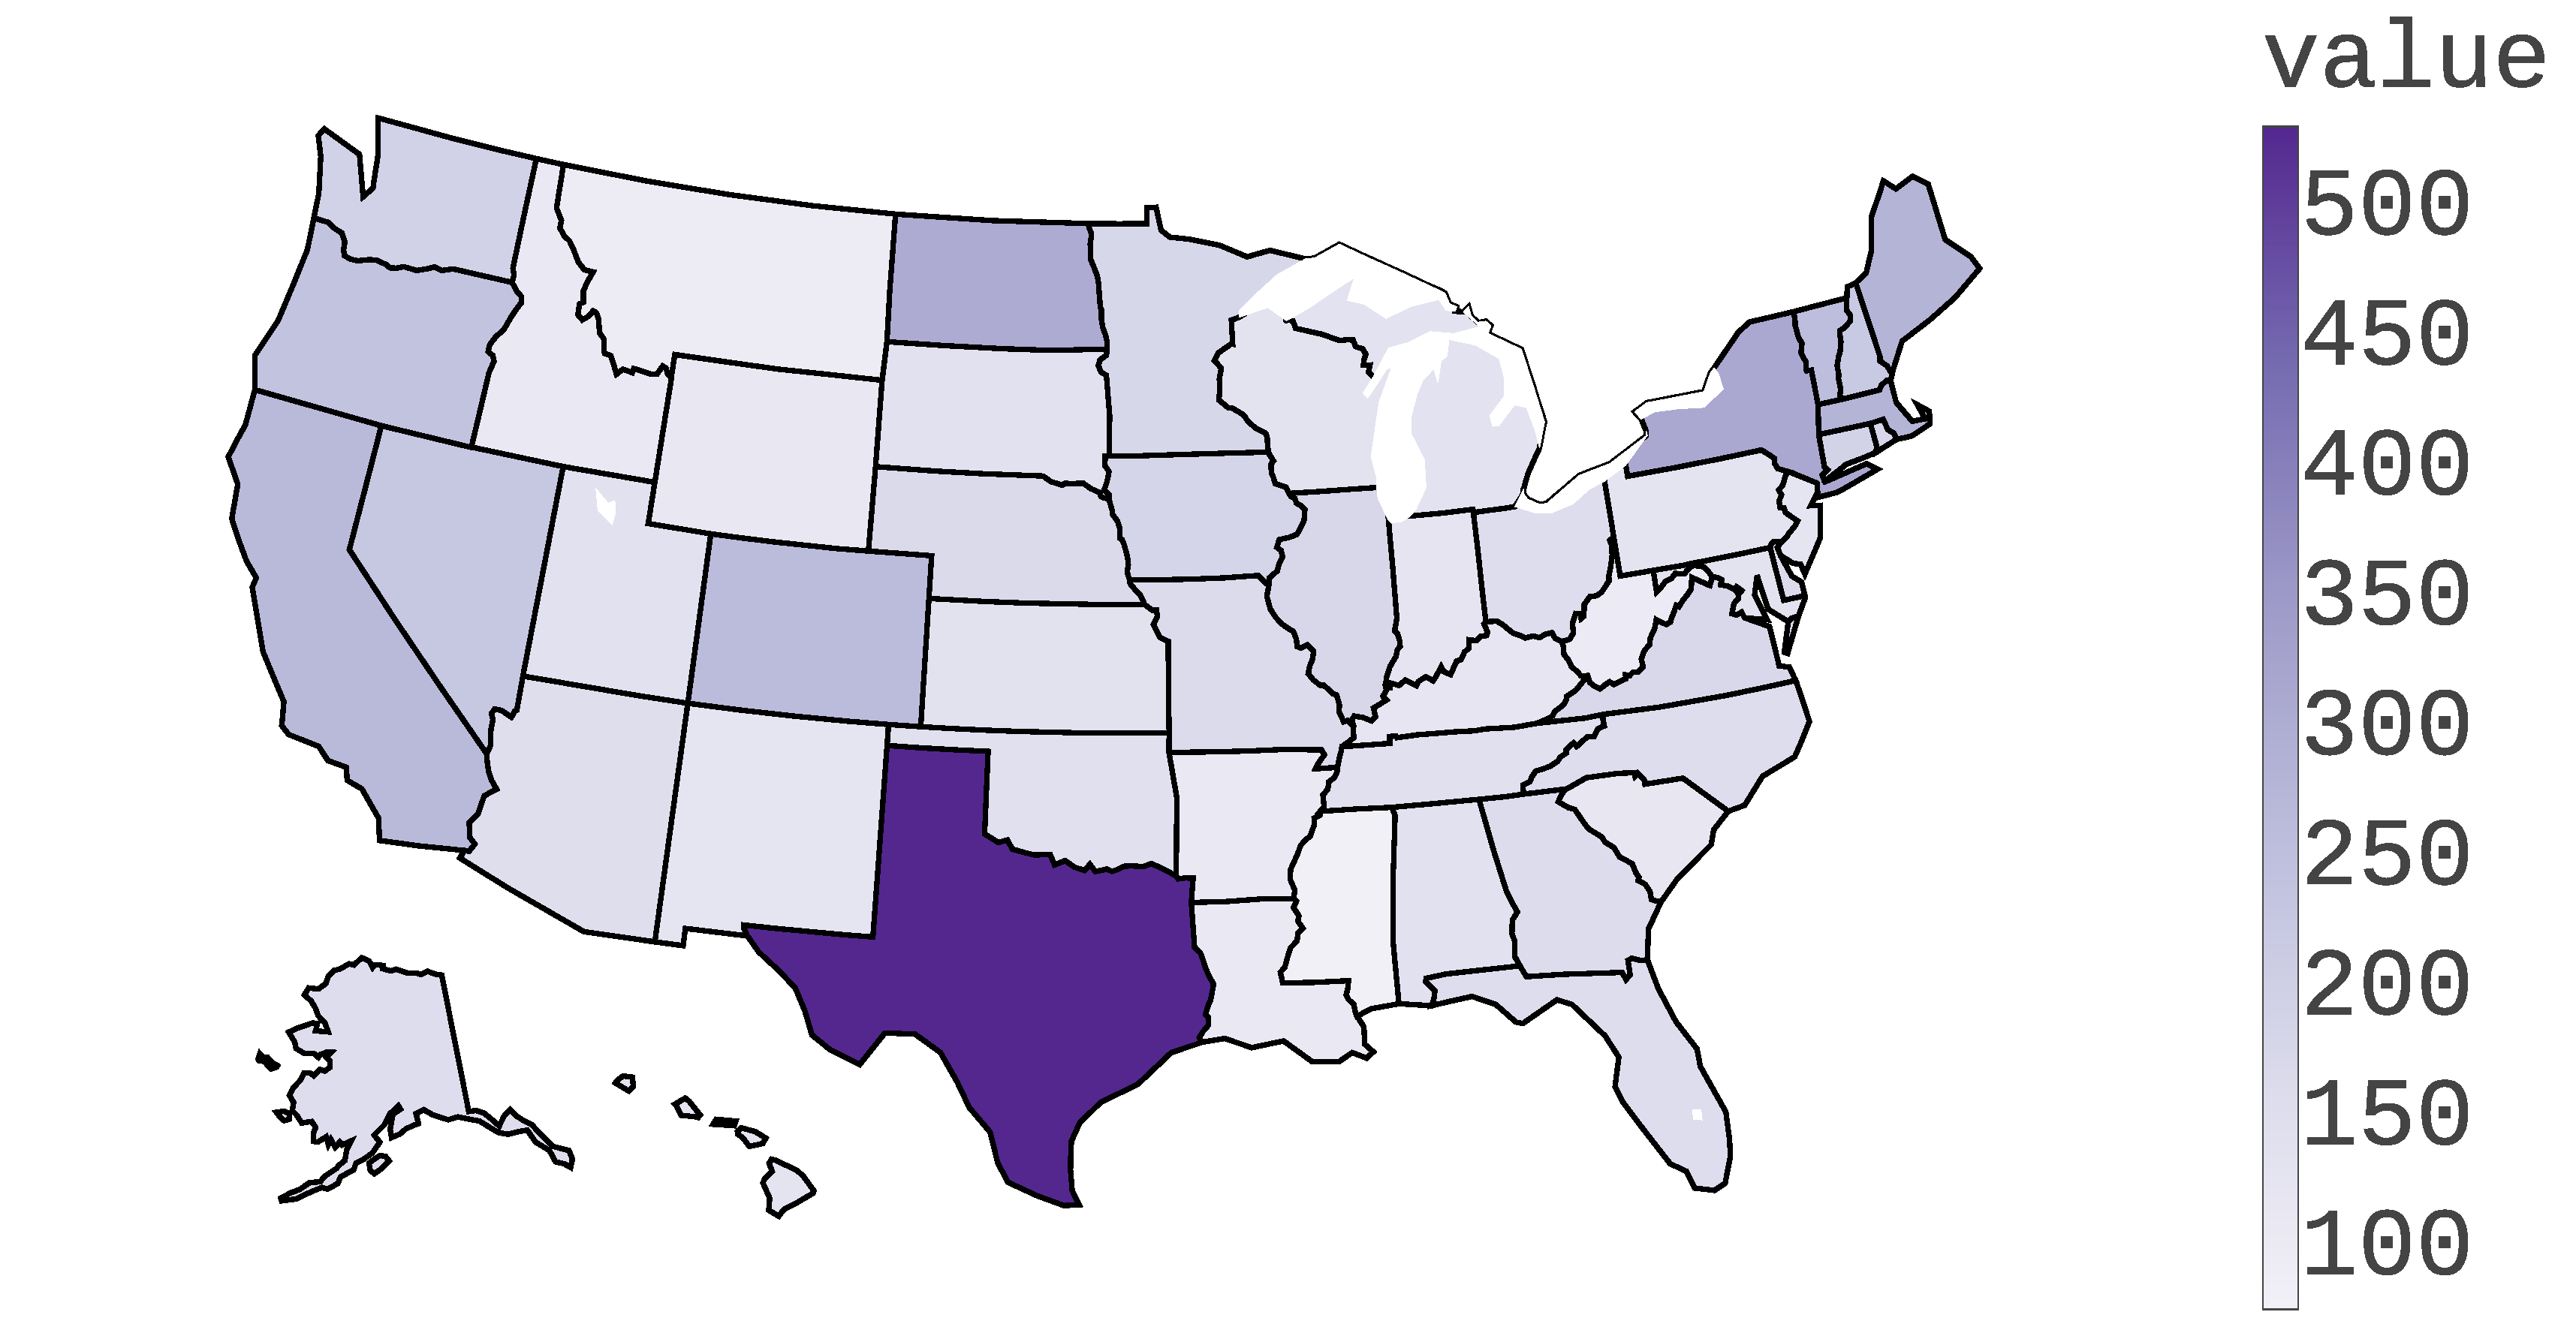
\includegraphics[width=5.3cm]{images/location/states/SocialSensor-us-states-space_location}} \\
\end{tabular}
\end{tabular}
\vspace{-2mm}
\caption {Distribution of tweets across International locations (top row) and U.S. locations (bottom row)}
\label{fig:choropleths}
\end{figure*}
%%%%%%%%%%%%%%%%%%%%%%%%%%%%%%%%%%%%%%%%%%%%%%%%%%%%%%%%%%%%%%%%%%%%%%%%%%%

Now we provide details of the Twitter testbed for topical social sensor learning
that we evaluate in this paper.  We crawled Twitter data using Twitter
Streaming API for two years spanning 2013 and 2014 years.
%This type of crawling provides us with a very sparse set of data, roughly $1\%$ of all tweets \footnote{\hyperref[]{http://allthingsd.com/20101110/twitter-firehose-too-intense-take-a-sip-from-the-garden-hose-or-sample-the-spritzer|}}. 
The total number of tweets collected is $829,026,458$. In the context
of Twitter, we consider five feature types for each tweet.  Each
tweet has a \textit{From} feature (i.e., the person who tweeted it), a
possible \textit{Location} (i.e., a string provided as meta-data), and
a time stamp when it was posted.  A tweet can also contain one or more
of the following:
\begin{itemize}
%NOTE: $$ is not for italics... it is for math mode and has larger math mode spacing
%since adjacent letters are implicitly multiplied.  Use \textit -SPS
\item \textit{Hashtag}: a topical keyword specified using the \# sign.
\item \textit{Mention}: a Twitter username reference using the @ sign. % reply?
\item \textit{Term}:    any non-hashtag and non-mention unigrams. %These uni-grams are later cleaned to remove $Term$s with no meaning (total number of $Term$s before cleaning was $20,234,729$)
\end{itemize}
We provide more detailed statistics about each feature in
Table~\ref{table:featureStatistics}.  For example,
authors (\textit{From} users) have used a median value of $2$
unique hashtags % not average, median!!! -SPS
and a hashtag has been used on average by $10.08$ unique users.

Fig.~\ref{fig:choropleths} shows per capita tweet frequency across
different international and U.S. locations for different topics.
While English speaking countries dominate English tweets, we
see that the Middle East and Malaysia additionally stand out for the
topic of Human Caused Disaster (MH370 incident), Iran and Europe
for the ``Iran deal'', and
soccer for many countries where it is popular.  For U.S. states,
we see that Colorado stands out for health epidemics (both whooping
cough and pneumonic plague), Missouri stands out for social issues
(\#blacklivesmatter in St. Louis), and Texas stands out for space due to
NASA's presence there.

%%%%%%%%%%%%%%%%%%%%%%%%%%%%%%%%%%%%%%%%%%%%%%%%%%%%%%%%%%%%%%%%%%
\begin{table}[t!]
\centering
{\renewcommand{\arraystretch}{1.2}
\resizebox{0.5\textwidth}{!}{%
\begin{tabular}{|c|c|c|c|c|}
%\hline
\multicolumn{5}{c}{\textbf{\#Unique Features}} \\ \hline
\textbf{From} & \textbf{Hashtag} & \textbf{Mention} & \textbf{Location} & \textbf{Term} \\ \hline
95,547,198 & 11,183,410 & 411,341,569 & 58,601 & 20,234,728 \\ \hline %14,197,509
\end{tabular}
}}
%\vspace{.5mm}
%\caption{Number of unique features for each type.}%values for each feature of $829,026,458$ tweets in our Twitter dataset}
%\label{table:featureUnique}
%\end{table}
%
%\begin{table}[t!]
%\centering
{\renewcommand{\arraystretch}{1.2}
\resizebox{0.5\textwidth}{!}{%
\begin{tabular}{|l|c|c|c|c|}
%\hline
\multicolumn{5}{c}{\textbf{Feature Usage in \#Tweets}} \\ \hline
\textbf{Feature} & \textbf{Max} & \textbf{Avg} & \textbf{Median} & \textbf{Max entity} \\ \hline
\textbf{From} & 10,196 & 8.67 & 2 & running\_status \\ \hline
\textbf{Hashtag} & 1,653,159 & 13.91 & 1 & \#retweet \\ \hline
\textbf{Mention} & 6,291 & 1.26 & 1 & null \\ \hline
\textbf{Location} & 10,848,224 & 9,562.34 & 130 & london \\ \hline
\textbf{Term} & 241,896,559 & 492.37 & 1 & rt \\ \hline 
\multicolumn{5}{c}{\textbf{Feature Usage by \#Users}} \\ \hline
\textbf{Hashtag} & 592,363 & 10.08 & 1 & \#retweet \\ \hline
\textbf{Mention} & 26,293 & 5.44 & 1 & dimensionist \\ \hline
\textbf{Location} & 739,120 & 641.5 & 2 & london \\ \hline
\textbf{Term} & 1,799,385 & 6,616.65 & 1 & rt \\ \hline %SHOULD BE FIXED
\multicolumn{5}{c}{\textbf{Feature Using \#Hashtags}} \\ \hline
\textbf{From} & 18,167 & 2 & 0 & daily\_astrodata \\ \hline
\end{tabular}
}}
\caption{Feature Statistics of our $829,026,458$ tweet corpus.} % in our Twitter dataset}
\label{table:featureStatistics}
\end{table}
%%%%%%%%%%%%%%%%%%%%%%%%%%%%%%%%%%%%%%%%%%%%%%%%%%%%%%%%%%%%%%%%%%
